\chapter{Autonomous Observing}
\label{chap:autonomous}
\chaptoc{}

% ########################################

\newpage
\section{Introduction}
\label{sec:autonomous_intro}
\begin{colsection}

Continuing the description of the GOTO Telescope Control System from \aref{chap:gtecs}, in this chapter I describe the secondary layer of programs written to enable GOTO to operate as a robotic observatory.
%
\begin{itemize}
    \item In \nref{sec:something} I outline the additional functionality added to G-TeCS in order to allow the telescope to operate autonomously.
    \item In \nref{sec:pilot} I describe the master control program that operates the telescope when in robotic mode.
    \item In \nref{sec:conditions} I detail how G-TeCS monitors the local conditions, and list the different flags used to judge if it is safe to observe.
    \item In \nref{sec:observing} I give an outline of how targets are observed by the robotic system. These topics are expanded further in following chapters.
\end{itemize}
%
All work described in this chapter is my own, and again is based on \citet{Dyer}.

\end{colsection}

% ########################################

\newpage
\section{Something}
\label{sec:something}
\begin{colsection}

% ~~~~~~~~~~~~~~~~~~~~

\begin{colsection}

\todo{This whole section needs to be reorganised}

The hardware control systems described in \aref{sec:hardware_control} provide the basic methods to control and operate the telescope. A human observer could run through a series of simple commands to open the dome, slew the mount to a given target, take exposures once there, and then repeat with other targets for the rest of the night. There is a limited autonomy provided by the dome daemon, so the dome will close in bad weather without the delay from a human sending the command, but even that can be disabled if desired. Fundamentally the software described in \aref{sec:hardware_control} provides a perfectly usable human-operated telescope control system. \gls{goto}, however, was always designed as a fully robotic installation, as described in \aref{sec:control_requirements}. Therefore an additional level of software is required, to take the place of the observer as the source of the commands to the daemons.

In \gls{gtecs}, as in the \gls{pt5m} system before it, the role of the observer is filled by a master control program called the pilot. The pilot decides what to observe, sends commands to the daemons, monitors the hardware and attempts to fix problems that may arise. The intention is that the pilot will fully replicate anything a trained on-site observer would be required to do. In order to manage this there are several auxiliary systems and additional support daemons that the pilot confers with. The conditions daemon monitors weather and other system conditions, the sentinel daemon listens for alerts and enters new targets into the observation database and the scheduler daemon which reads that database and calculates what to observe. Each of these systems are described in the following sections.

\end{colsection}

% ~~~~~~~~~~~~~~~~~~~~

\subsection{Scripts}
\label{sec:scripts}
\begin{colsection}

As well as the daemons, the \pkg{gtecs} package includes multiple Python scripts. Once installed these scripts can all be run from the command line by a human, called from within other scripts like the pilot or run automatically with utilities like cron.

In order to send commands to the daemons each has an associated control script that can be called by a user from a terminal, or by the pilot in robotic mode (see \aref{sec:pilot}). The commands follow a simple format which was inherited from \gls{pt5m}, first the short name of the daemon, then the command and finally any arguments. There are several commands that are common to all daemons: \code{start}, \code{shutdown} and \code{restart} to control if the daemon is running; \code{ping} to see the current status of the daemon; \code{info} to see the current status of the hardware; \code{log} to print the daemon output log. Examples of daemon-specific commands include ``\code{dome~close}'' to close the dome, ``\code{mnt~slew~30.54~+62}'' to slew the mount to the given coordinates, ``\texttt{cam~image~60}'' to take a \SI{60}{\second} exposure with all connected cameras and ``\texttt{cam~image~2~60}'' to take a \SI{60}{\second} exposure with camera 2 only.

Every daemon can also be controlled in ``interactive mode'', which is a user-friendly way to save time sending multiple commands to the same daemon. Interactive mode is entered with \code{i} and exited with \code{q}.

There is also a utility script, \code{lilith}, which can send the same command to all the daemons. For example, to shutdown every daemon it is possible to call each directly (\code{cam shutdown}, \code{foc shutdown}, \code{mnt shutdown} etc\ldots) but it is instead much easier to run \code{lilith shutdown}. The name ``Lilith'' comes from the biblical ``mother of demons''.

The most important script to the robotic operation of the telescope is the pilot, detailed in \aref{sec:pilot}. The pilot is started every night using cron at 5pm, but can also be started manually with the command \code{pilot start} (note although this uses the same syntax as a daemon it simply runs the pilot script in the current terminal instead of starting a background process). There is also a daytime counterpart to the pilot, called the day marshal, which is run in the same way. Finally within the pilot, several of the standard tasks are separated off into ``observation scripts'', lists of commands to the daemons to carry out tasks like focusing the telescope, taking flat fields or starting/shutting down the hardware in the evening/morning respectively. As standard tasks these can also be run by human observers though a command line script \code{obs\_script} (for example \code{obs\_script~startup} or \code{obs\_script~autofocus}).

\end{colsection}

% ~~~~~~~~~~~~~~~~~~~~

\subsection{System mode}
\label{sec:mode}
\begin{colsection}

\gls{goto} is a robotic telescope, and \gls{gtecs} is designed around that concept. This means the system will operate nightly with no human intervention needed. However, sometimes it is necessary for a human operator to take control of the telescope, if one of the automated scripts fails or a situation arises that is easer to deal with manually. One example was taking observations of the asteroid Phaethon \citep{Phaethon}: G-TeCS was not designed to observe solar system objects, and although the mount allows sidereal tracking there was no way to add a pointing into the database without fixed coordinates. Therefore it was necessary for a human observer to look up and slew to the coordinates of the asteroid as it moved past the Earth. There are also cases when it is important that the automated systems are disabled: if work is being done to the hardware on-site it could be dangerous if the system still tried to move the mount or dome autonomously.

\begin{table}[t]
    \begin{center}
        \begin{tabular}{c|ccccc} % chktex 44
            mode &
            pilot &
            day marshal &
            dome autoclose &
            dome alarm &
            \code{hatch} flag
            \\
            \midrule
            \code{robotic} &
            \textcolor{Green}{active} &
            \textcolor{Green}{active} &
            \textcolor{Green}{enabled} &
            \textcolor{Green}{enabled} &
            \textcolor{Green}{active}
            \\[5pt]
            \code{manual} &
            \textcolor{Orange}{paused} &
            \textcolor{Green}{active} &
            \textcolor{Orange}{adjustable} &
            \textcolor{Orange}{adjustable} &
            \textcolor{Red}{ignored}
            \\[5pt]
            \code{engineering} &
            \textcolor{Red}{disabled} &
            \textcolor{Red}{disabled} &
            \textcolor{Red}{disabled} &
            \textcolor{Red}{disabled} &
            \textcolor{Red}{ignored}
            \\
        \end{tabular}
    \end{center}
    \caption[System mode comparison]{
        A comparison of the three \gls{gtecs} system modes. In \code{robotic} mode all of the automated systems are enabled, in \code{engineering} mode they are all disabled, and in \code{manual} mode the pilot is paused and the observer can disable the dome systems if desired.
    }\label{tab:modes}
\end{table}

\gls{gtecs} deals with manual operation by having an overall system mode flag stored in a datafile which is checked by the automated systems before activating. There are three possible modes, outlined below and summarised in \aref{tab:modes}.

\begin{itemize}
    \item \code{robotic} mode is the default mode for the telescope. In this case it is assumed that the system is completely automated and therefore could move at any time. In this mode during the night the pilot will be in complete control of the telescope, and the dome will automatically close in bad weather. The dome hatch being open is also treated as a critical conditions flag (see \aref{sec:conditions}).

    \item \code{manual} mode is designed for manual observing, either on-site or remotely. In this mode the pilot will be paused and so will not interrupt commands sent by the observer. The dome will still sound the alarm when moving and autoclose in bad weather by default, but both of these features can be disabled; it is intended that they should only be disabled if there is an observer physically present in the dome, otherwise the dome should still be able to close automatically when observing remotely.

    \item \code{engineering} mode is designed to be used only if there are workers on site in situations where the system moving without warning could be dangerous. All of the dome options are automatically disabled, and the pilot and day marshal will refuse to start. Leaving the system in this state for long periods of time is undesirable, and so it should only be used when physical work is ongoing or the telescope is completely deactivated.
\end{itemize}

\end{colsection}

% ~~~~~~~~~~~~~~~~~~~~

\end{colsection}

% ########################################

\newpage
\section{The pilot}
\label{sec:pilot}
\begin{colsection}

% ~~~~~~~~~~~~~~~~~~~~

\begin{colsection}

The pilot is a Python script, \code{pilot.py}, not a daemon. It is run once each night; started automatically in the late afternoon by the Linux cron utility, it runs through to the morning and then quits. In the afternoon it will be started again and the process will be repeated.

\end{colsection}

% ~~~~~~~~~~~~~~~~~~~~

\subsection{Asynchronous code}
\label{sec:async}
\begin{colsection}

The pilot is written as an \textit{asynchronous} program, using the standard Python module AsyncIO (\pkg{asyncio}). An asynchronous program is one where its code runs in separate parallel routines, which are switched between as required, and should not be confused with programs that are written utilising multiple processes or threads that run in parallel. See \aref{fig:async} for a graphical comparison between the two methods.

An example of a simple task might be monitoring a particular source of data, like a weather station. It would contain a function to download the current weather information from the external mast, and then a \code{sleep} command to wait for 10 seconds, which when put inside a loop will ensure that the weather information is queried and updated every 10 seconds. If this loop was called in a multi-threaded program then the thread will be held up for a majority of the time not doing anything between checks. If there were multiple threads, for example checking different masts, then there could be no coordination between them and the whole program would end up being very inefficient. There are also other issues with multi-threaded programs, including input/output and sharing data between threads.

Asynchronous code contains multiple parallel \textit{coroutines}. The program itself runs an \textit{event loop}, which is a function with the job of choosing between the different coroutines to execute in the main thread. In an asynchronous version of the weather-monitoring program instead of a \code{sleep} function each coroutine would include an \code{await} function. When a routine reaches an \code{await} command it is suspended for the given time period, and control is passed back to the event loop which then chooses which of the other suspended routines should be run. Importantly when it resumes the coroutine remembers where it stopped and continues from that point. The asynchronous style of writing code is ideally used with multiple coroutines that contain short functions with wait periods between when they need to be called again, and the pilot is a good example of this. The pilot runs a single-threaded event loop with multiple coroutines, which execute commands and then pause using the \texttt{await} command to allow other routines to be run.

\begin{figure}[p]
    \begin{center}
        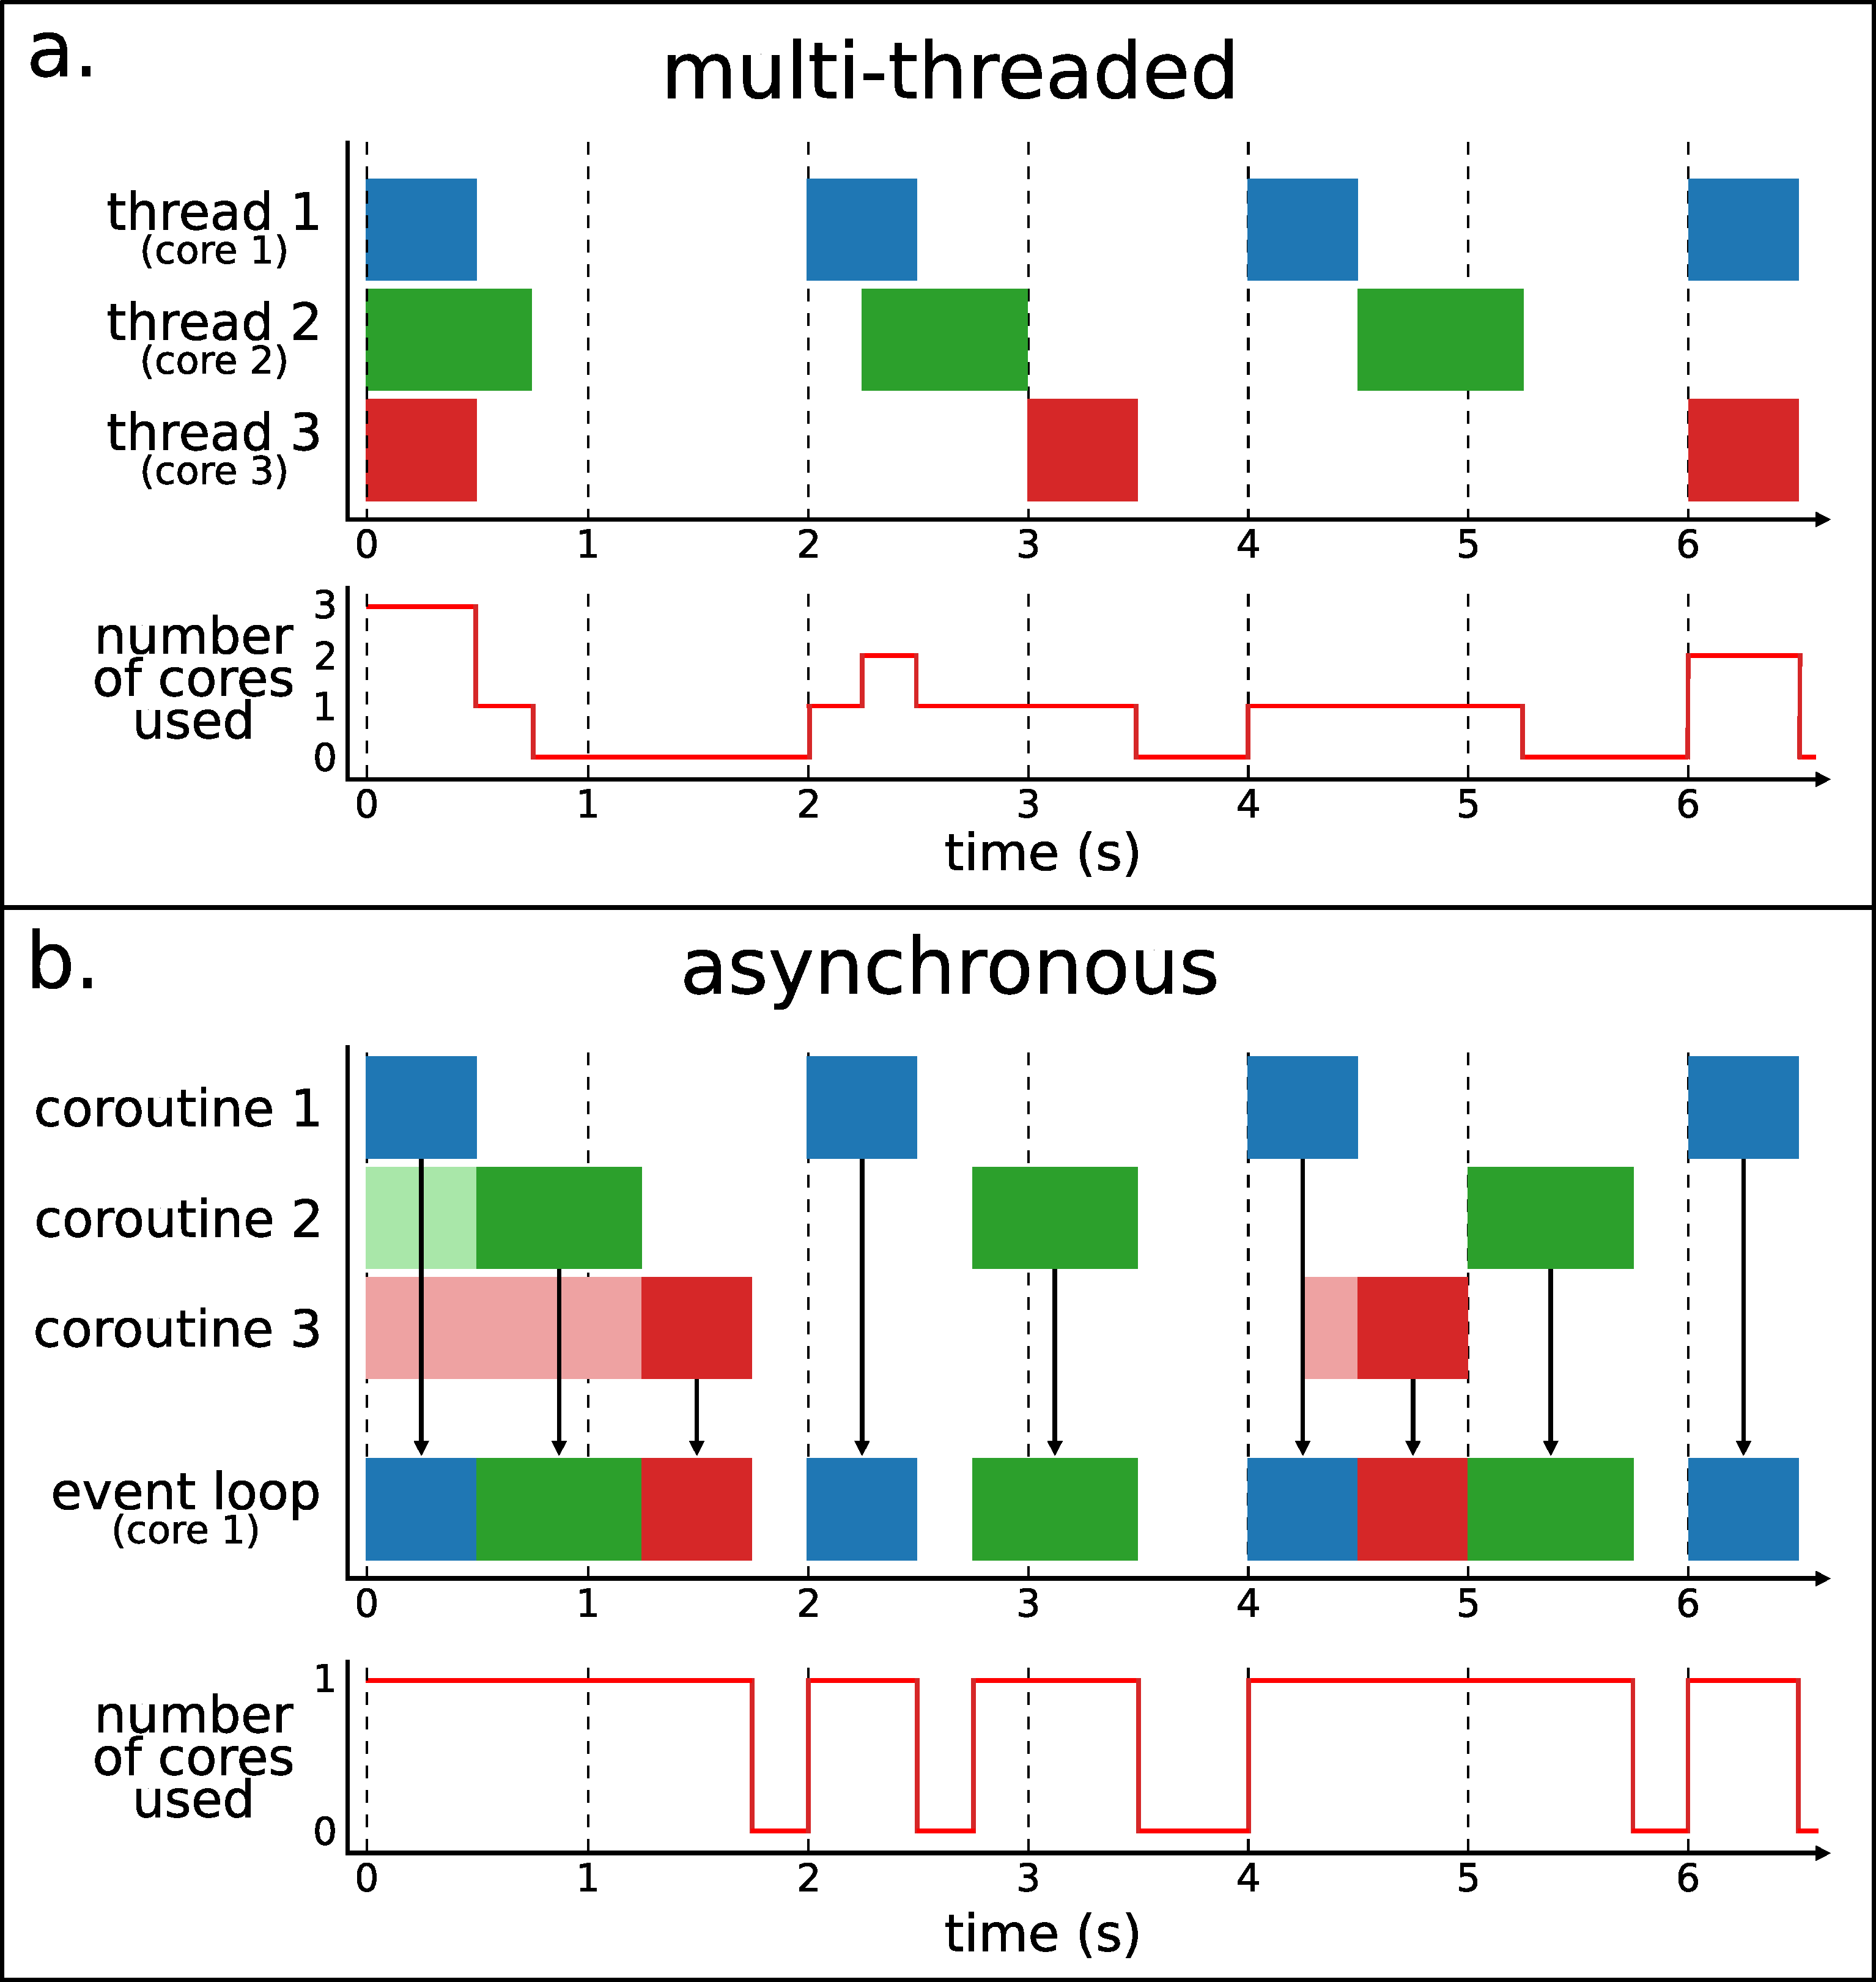
\includegraphics[width=0.89\linewidth]{images/async.pdf} % TODO:recolour
    \end{center}
    \caption[Multi-threaded vs asynchronous programming]{
        A comparison of multi-threaded vs asynchronous programming. This example uses a \textcolorbf{NavyBlue}{blue} task that takes \SI{0.5}{\second} to execute and then waits for \SI{1.5}{\second}, a \textcolorbf{Green}{green} task that takes \SI{0.75}{\second} and waits for \SI{1.5}{\second} and a \textcolorbf{Red}{red} task that takes \SI{0.5}{\second} and waits for \SI{2.5}{\second}. These times are exaggerated for clarity, pilot tasks typically take less than a second and wait for between 10 and 60 seconds. \\
        \textbf{Top}: The three tasks with different execution periods (solid blocks) and wait times (blank) are run in a multi-threaded program. Each task is being run in an independent parallel thread on its own core, even though they rarely overlap and it is uncommon for multiple cores to be in use at the same time. \\
        \textbf{Bottom}: The same three tasks are run as coroutines in an asynchronous program. The event loop decides which coroutine to run on the single core, represented by the black arrows. This does lead to some coroutines being left waiting (lighter blocks) until the previous is finished, and as routines can be delayed it is not suitable for checks that need to happen at exact frequencies. However the overall core usage is much more efficient.
    }\label{fig:async}
\end{figure}

\end{colsection}

% ~~~~~~~~~~~~~~~~~~~~
\subsection{Check routines}
\label{sec:checks}
\begin{colsection}

The coroutines within the pilot can be separated into two types: the check routines and the night marshal. Most of the coroutines are designed as monitors to regularly check different parts of the system, which fits well into the asynchronous model. These check routines are as follows:

\begin{itemize}

\item \texttt{check\_flags} is a routine that monitors the system flags, most notably those created by the conditions daemon (see \aref{sec:conditions}). If any of the conditions flags are bad then the dome daemon will enter lockdown and close the dome on its own (see \aref{sec:dome}), but the \texttt{check\_flags} routine will abort exposures, pause the pilot and ensure it is not resumed until the flag is cleared. When the pilot is paused the dome will close, the mount will park, and the night marshal (see below) will not trigger any more tasks. When conditions are clear again the pilot will reopen the dome and allow normal operations to be restored. The \texttt{check\_flags} routine also monitors the system mode and will pause the pilot if it is set to manual mode or exit if set to engineering mode (see \aref{sec:mode}).

\item \texttt{check\_scheduler} is a routine that queries the scheduler daemon (see \aref{sec:scheduler}) every 10 seconds to find the best job to observe. If the pilot is currently observing the scheduler will either return the database ID of the current pointing, in which case the pilot will continue with the current job, or a new ID which will lead to the pilot interrupting the current job and moving to observe the new one. If the pilot is not currently observing (either it is the start of the night, resuming from being paused or the previous pointing has just completed) then it will begin observing whatever the scheduler returns. The details of how the scheduler decides which target to observe are given in \aref{sec:scheduler}. The ID returned is then passed to the observe (OBS) task run by the night marshal (see below).

\item \texttt{check\_hardware} monitors the hardware daemons (see \aref{sec:hardware_control}), checking every 60 seconds that they are all reporting their expected statuses. It does this using the hardware monitor functions, which are described below. If an abnormal status is returned then the pilot will pause and a series of pre-set recovery commands generated by the monitor are executed in turn. While in recovery mode the pilot will check the monitors more frequently. If the commands work and the status returns to normal the pilot is resumed, but if the commands are exhausted without the problem being fixed then an alert is issued that the system requires human intervention and the pilot triggers an emergency shutdown.

\item \texttt{check\_dome} is a backup to the primary hardware check routine. \texttt{check\_hardware} does monitor the dome along with the other hardware daemons, but \texttt{check\_dome} provides a simple, dedicated backup to ensure the dome is closed when it should be and to raise the alarm if it is not.

\end{itemize}

\end{colsection}

% ~~~~~~~~~~~~~~~~~~~~
\subsection{Monitoring the hardware}
\label{sec:monitors}
\begin{colsection}

One of the important tasks that the pilot is required to do is monitoring the status of the various system daemons, and therefore the hardware units they are connected to. If any problems were detected the easiest automated response would be to shutdown everything and send a message for a human to intervene. However this would be unnecessary in the case of small problems that could be easily fixed with one command, and it would be much better if the pilot could identify the problem and issue the command itself. The other benefit of this is a much faster reaction time than potentially needing to wake a human operator in the middle of the night, this is important both to minimise observing time lost and also potentially save the hardware by, for example, making sure the dome is closed in bad weather.

Therefore a system was created to enable the pilot to attempt to respond and fix any errors that occur itself. This is done within the \code{check\_hardware} coroutine though a series of hardware monitor Python classes, one for each of the daemons (i.e. \code{DomeMonitor}, \code{CamMonitor} etc.). Each daemon has a set of recognised statuses, representing the current hardware state, and a set of valid modes which represent the expected state. The current status is fetched from the hardware daemon, the mode is set by the pilot, and the hardware checks consist of comparing the two to discover if there are any inconsistencies. For example, the dome daemon can have current statuses of \code{OPEN}, \code{CLOSED} or \code{MOVING}, and its valid modes are just \code{OPEN} and \code{CLOSED}. At the start of the night when the pilot starts the dome should be in \code{CLOSED} mode, and the pilot only switches it to \code{OPEN} mode when it is ready to open the dome. If when a check is carried out the dome is in \code{CLOSED} mode but the current status is reported as not \code{CLOSED} then that is a problem, and the hardware check function returns that it has detected an error with the dome. These checks can have timeouts associated with each status. For example if the dome is in \code{CLOSED} mode and is reported as \code{MOVING} that is not necessarily an error, as it might be currently closing. The hardware monitor stores the time since the hardware status last changed, so if the dome reports that it has been in the moving state for longer than it would take to close then that raises an error. This example used states specific to that hardware, but every daemon also has various other possible states and errors --- for example if the daemon is not running, or is running and not responding.

When one of the monitor checks returns an error then the pilot will take action as described within the \code{check\_hardware} routine: pause night marshal (see below), stop any current tasks and send a Slack alert to record the error. But instead of stopping there, the monitor goes on to attempt to recover from the error and fix the problem. In the same way that a human observer would run though a series of commands in order to solve the problem, each monitor has a defined set of recovery steps to be run through depending on the error reported. Continuing with the previous example, if the dome reports \code{OPEN} when in \code{CLOSED} mode then the first recovery step is simple: execute the command \code{dome~open}. Each step then has a timeout value and an expected state if the recovery command worked. If after 10 seconds the status of the dome has not changed from \code{OPEN} to \code{MOVING}, then the error is persisting and more actions need to be taken. If however the dome daemon reports that the dome is moving then the error is not cleared immediately, only when the status finally reaches \code{CLOSED}. As mentioned previously, should a monitor run out of recovery steps then the pilot will send out an alert that there is nothing more that it can do and will attempt an emergency shutdown.

Using the above method, the vast majority of hardware issues can be solved by the pilot without the need for human intervention. Every time the recovery steps are triggered a message is sent to Slack detailing the error and the steps required to fix it, so it is easy to then go back and examine why the error occurred and how to prevent it in the future.

\end{colsection}

% ~~~~~~~~~~~~~~~~~~~~
\subsection{The night marshal}
\label{sec:night_marshal}
\begin{colsection}

The above check routines are support tasks for the primary routine, which is called the \texttt{night\_marshal}. Unlike the check routines the night marshal does not contain a loop, instead it runs through a list of tasks as the night progresses, based on the altitude of the Sun. Each task is contained in a separate Python observation script, which contains the commands to send to the hardware daemons. These scripts are self-contained programs which mean they can also be called independently, for example if the pilot is not running and a manual observer wants to run the autofocus routine they can use the command \texttt{obs\_script~autoFocus}. Each is run by spawning a new coroutine, meaning that while they are running the other routines such as the check tasks can continue. In the order they are performed during the night, the night marshal tasks are:

\begin{enumerate}

\item STARTUP, run immediately when the pilot starts. The \texttt{startup} script powers on the camera hardware, unparks the mount, homes the filter wheels and cools the CCDs down to their operating temperature of \SI{-20}{\celsius}. Once startup has finished the pilot will send a report of the current conditions to Slack (see \aref{fig:pilot_slack} below).

\item DARKS, run after the system start up is complete before opening the dome. This executes the \texttt{takeBiasesAndDarks} script to take bias and dark frames at the start of the night. \todo{see commissioning}

\item OPEN, run once the Sun reaches \SI{0}{\degree} altitude. It simply executes the \texttt{dome~open} command. If the pilot is paused due to bad weather or a hardware fault then the night marshal will wait and not open until the weather improves or fault is fixed. If it is never resolved then the night marshal will remain at this point until the end of the night and the shutdown timer runs out (see below).

\item FLATS, run once the dome is open and the Sun reaches \SI{-1}{\degree}. This executes the \texttt{takeFlats} script, which moves the telescope into a position pointing away from the Sun and then takes flat fields in each filter, stepping in position between each exposure and automatically increasing the exposure time as the sky darkens. See \aref{sec:flats} for details of the flat field routine.

\item FOCUS, run once the Sun reaches \SI{-11}{\degree}. This executes the \texttt{autoFocus} script, which finds the best focus position for each of the unit telescopes. See \aref{sec:autofocus} for details of the autofocus routine. If the routine fails for any reason the previous nights' focus positions are restored.

\item OBS (short for ``observing''), begun once the Sun reaches \SI{-15}{\degree} and continuing for the majority of the night until the Sun reaches \SI{-15}{\degree} again in the morning. When a database ID is received from the scheduler via the \texttt{check\_schedule} routine the \texttt{observe} script is executed. The script queries the observation database (see \aref{sec:obsdb}) to get the coordinates and exposure settings for that pointing and then sends the commands to the mount and exposure queue daemons. Once a job is finished, either through completing all of its exposures or being interrupted, the entry in the database is updated and the routine starts observing the next job from the scheduler.

\item FLATS is repeated once the Sun reaches \SI{-10}{\degree} in the morning, using the same script but this time increasing the exposure times as the sky brightens.

\end{enumerate}

Once the night marshal has completed all of its tasks it exits and triggers the \texttt{shutdown} script, which powers off the cameras, parks the mount and ensures the dome is closed. Once this is finished the pilot quits. In addition there is a separate night countdown timer within the pilot, which will trigger the shutdown if the Sun ever reaches \SI{0}{\degree}. Normally the night marshal will have finished and triggered the shutdown long before that point, but the countdown acts as a backup ensuring that if there is a problem with the night marshal the pilot will still trigger a shutdown.

It is also possible for the pilot to trigger an emergency shutdown during the night. This triggers the same \texttt{shutdown} script observing script, with the only difference being that it ensures the dome is closed first. An emergency shutdown will be triggered by the pilot only in situations that it could not recover from without human intervention, notably if the \code{check\_hardware} routine reaches the end of a daemon's recovery steps without solving the problem.

\end{colsection}

% ~~~~~~~~~~~~~~~~~~~~
\subsection{The day marshal}
\label{sec:day_marshal}
\begin{colsection}

The day marshal is another script that provides a counterpart to the pilot (the mirror of the night marshal within the pilot). The \code{day\_marshal.py} script is run as a cron job like the pilot, but starts in the early morning rather than the late afternoon. The day marshal is a much simpler script, with only one key task --- to wait until dawn and then check that the dome is closed. In this sense it is yet another backup to the pilot's inbuilt \code{night\_countdown} timer, and as it is completely independent of the pilot it will run even if the pilot has crashed. Should it find that the dome is still open then the script will continuously try closing it, and send out human alerts that the system has failed. The day marshal will also send out a Slack report, again as a mirror of the report that the night marshal sends after startup, to confirm that the dome is closed.

\end{colsection}

% ~~~~~~~~~~~~~~~~~~~~
\subsection{Slack alerts}
\label{sec:slack}
\begin{colsection}

Although the pilot is a completely robotic system it is still important that it doesn't operate completely unsupervised. As the \gls{goto} collaboration has adopted the Slack messaging client\footnote{\url{https://slack.com}} for instant messaging and collaboration it was decided that the telescope control system should send reports automatically to a dedicated Slack channel. This was implemented through the Python Slack \gls{api} module \pkg{slackclient}, and has been widely adopted throughout G-TeCS.\@ The two most complicated Slack messages are the startup report, sent by the night marshal within the pilot, and the morning report sent by the day marshal. The startup report includes a summary of the current condition flags, links to the site weather pages, the external webcam view and the latest IR satellite image over La Palma. The morning report includes the internal webcam view and plots showing what tiles the pilot observed last night and the current status of the all-sky survey. Examples of both are shown in \aref{fig:pilot_slack}. Several other functions send short reports, for example when the pilot starts and stops, when the dome opens and closes, if the system mode changes, or if a hardware error is being fixed. The pilot sends a majority of the messages to Slack but other daemons do as well, including the dome daemon when it enters lockdown (see \aref{sec:dome}) and the sentinel when it processes an interesting alert through GOTO-alert (see \aref{sec:sentinel} and \aref{sec:event_slack}).

\begin{figure}[p]
    \begin{center}
        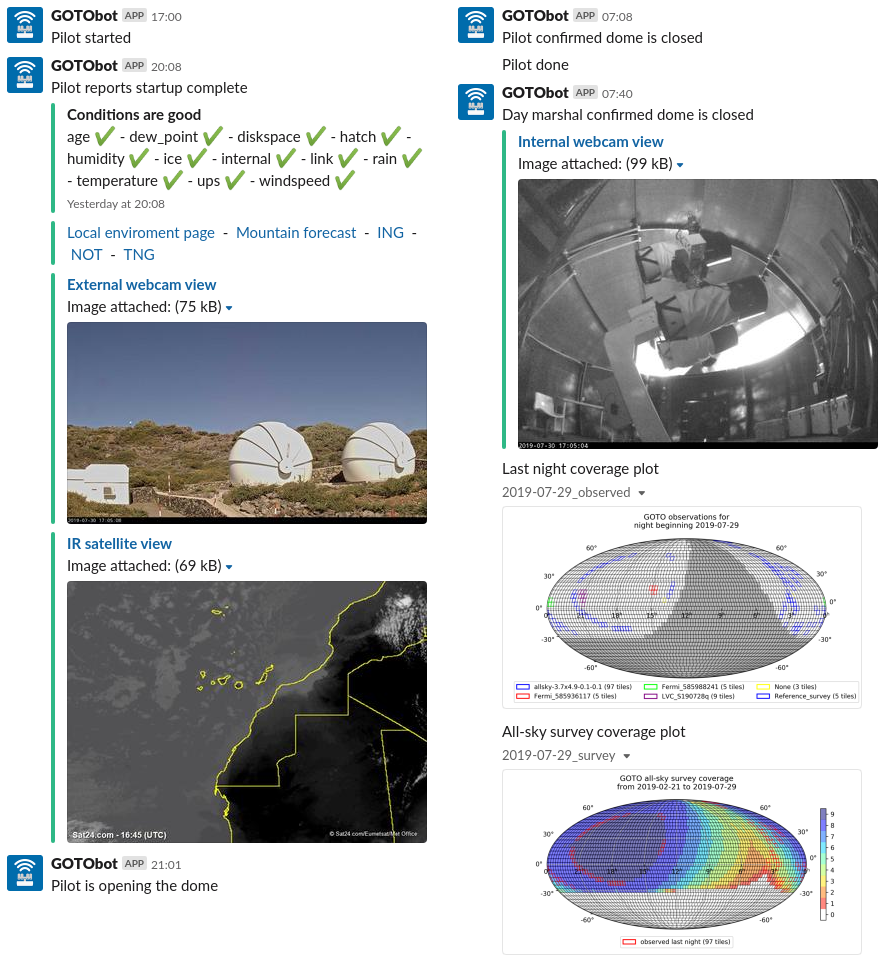
\includegraphics[width=\linewidth]{images/slack2.png}
    \end{center}
    \caption[Slack messages sent by the pilot and day marshal]{
        Slack messages sent by the pilot and day marshal on a typical night. The pilot reports when it starts automatically at 5pm, then the night marshal sends out the startup report when the STARTUP task has completed. The pilot also sends out messages when it is opening and closing the dome, and when it finishes in the morning. The day marshal later independently confirms the dome is closed and sends out its own morning report.
    }\label{fig:pilot_slack}
\end{figure}

\end{colsection}

% ~~~~~~~~~~~~~~~~~~~~

\end{colsection}

% ########################################

\newpage
\section{Conditions monitoring}
\label{sec:conditions}
\begin{colsection}

% ~~~~~~~~~~~~~~~~~~~~

\begin{colsection}

\todo{Monitoring the conditions is important}
\todo{Maybe a map of the site? Brief overview of weather in La Palma?}

\begin{figure}[t]
    \begin{center}
        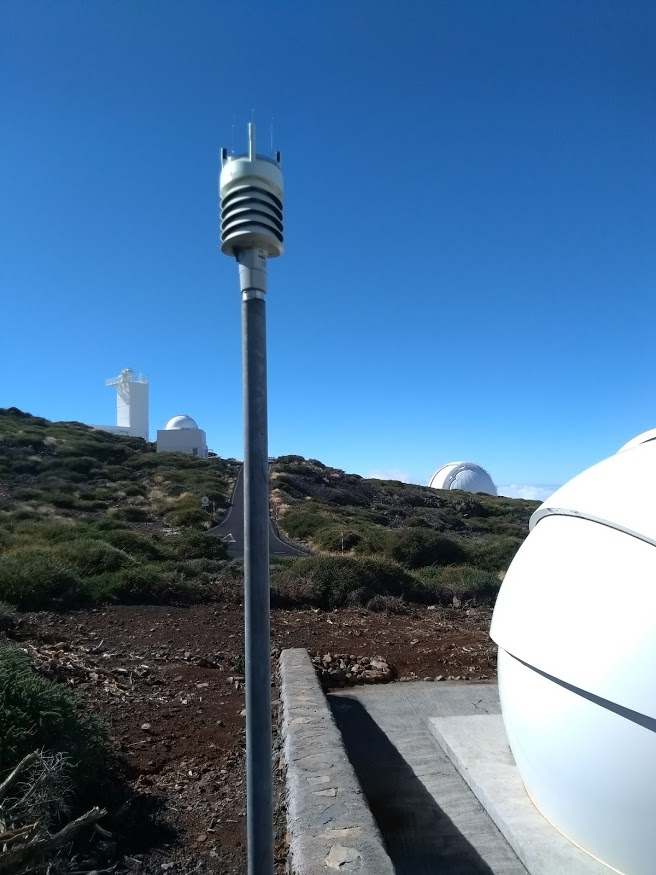
\includegraphics[width=0.3\textwidth]{images/conditions_photo.jpg}
        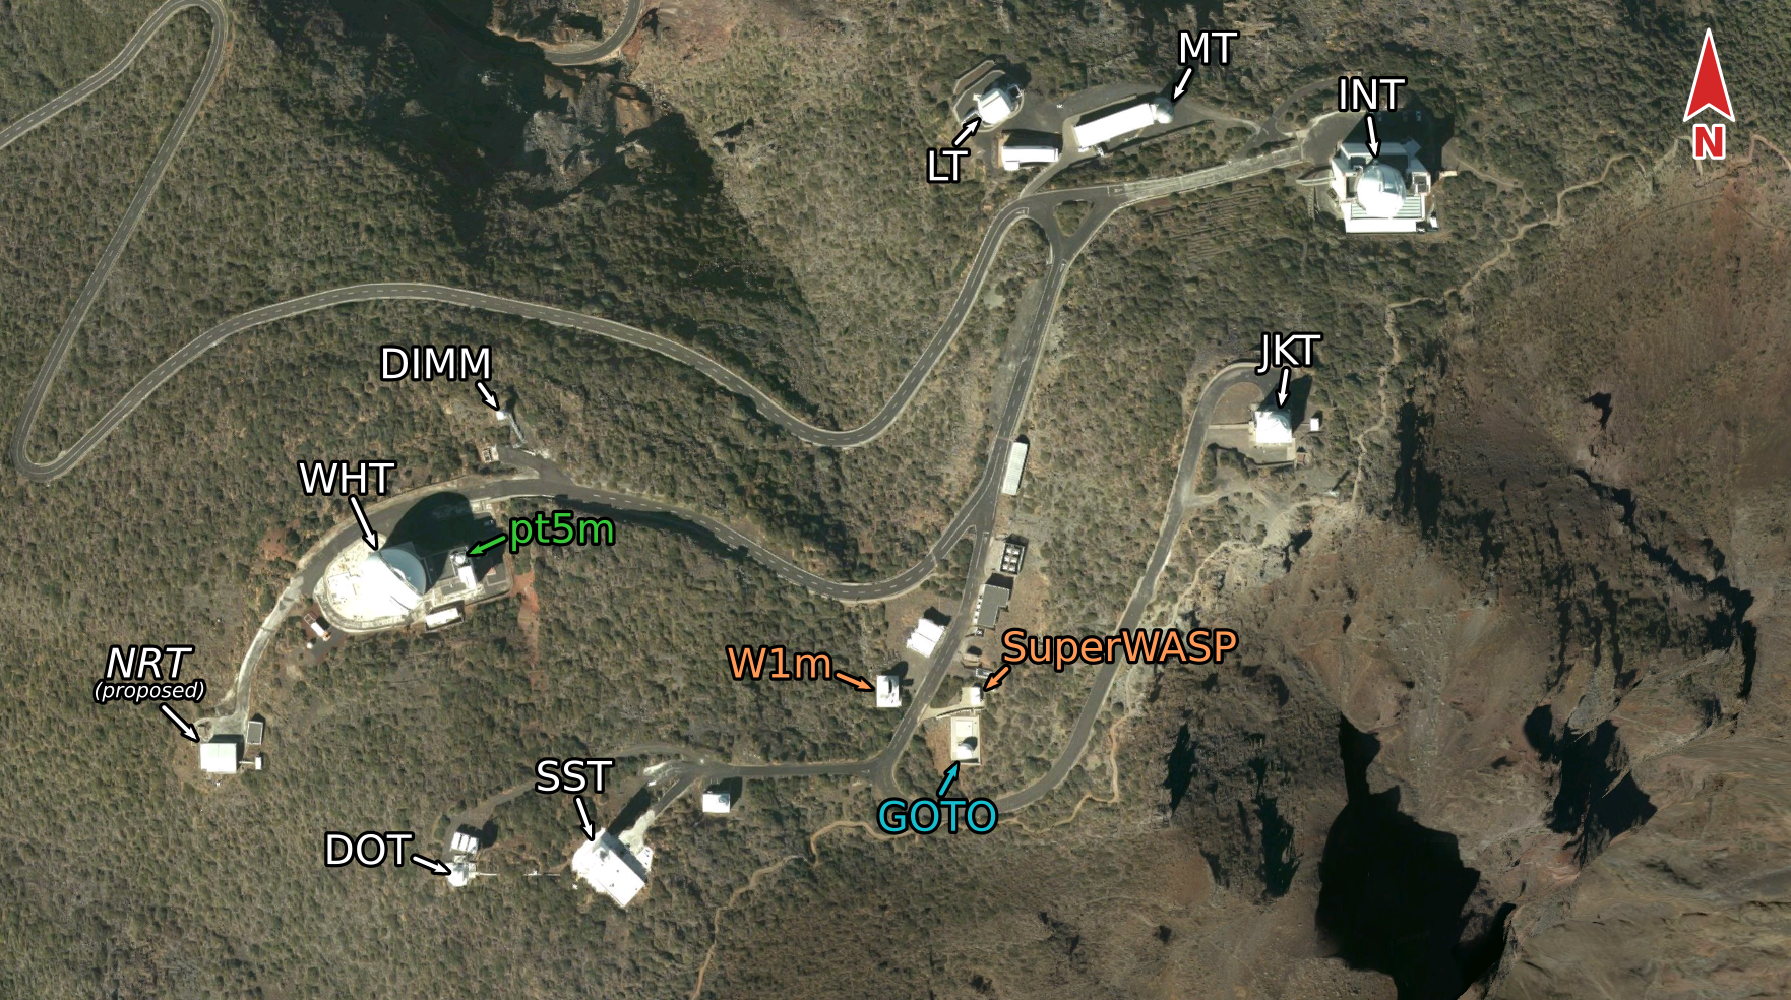
\includegraphics[width=0.5\textwidth]{images/orm_east_labelled.png}
    \end{center}
    \caption[\todo{todo}]{
        \todo{todo}.
    }\label{fig:conditions}
\end{figure}

\end{colsection}

% ~~~~~~~~~~~~~~~~~~~~
\subsection{The conditions daemon}
\label{sec:conditions_daemon}
\begin{colsection}

The conditions daemon is a support daemon that runs on the central observatory server in the SuperWASP building on La Palma (see \aref{fig:flow}). It takes in readings from the three local weather stations next to the GOTO dome on La Palma, as well as other sources such as internal sensors, every 10 seconds. The daemon processes these inputs into a series of output flags, which have a value of \code{0} (good), \code{1} (bad) or \code{2} (error). If any of the flags are marked as not good (i.e.\ the sum of all flags is $>0$) then the overall conditions are bad: the dome will enter lockdown and automatically close if it is open (see \aref{sec:dome}) and the pilot \code{check\_flags} routine will trigger the pilot to pause observations (see \aref{sec:pilot}). The conditions daemon is run on the central server because it deals with site-wide values, so when the second GOTO telescope on La Palma is built it is envisioned that they will both share the same conditions daemon (see \aref{sec:gtecs_multisite}).

\end{colsection}

% ~~~~~~~~~~~~~~~~~~~~
\subsection{Conditions flags}
\label{sec:conditions_flags}
\begin{colsection}

Each conditions flag has a limit below or above which the flag will turn from good to bad. For categories with multiple sources (for example there are three local weather stations, located at GOTO, SuperWASP and W1m, and each gives an independent external temperature reading) then the limit will be applied to each and if \textit{any} are found to be bad then the flag is set. If follows therefore that \textit{all} the conditions sources must be good for the flag to be set to good. Each category also has two parameters, the bad delay and the good delay. These are the time the conditions daemon waits between an input going bad/good and setting the flag accordingly, which has the effect of smoothing out any sudden spikes in a value and ensures the dome will not be opening and closing too often.

The conditions flags can be grouped into three categories, divided according to severity. The latest version of G-TeCS contains 13 flags, listed in \aref{tab:conditions_flags}. An explanation of the different categories, and the flags within each, is given below.

\begin{table}[p]
    \begin{center}
        \begin{tabular}{c|cccc} % chktex 44
            Flag name           & Criteria measured & Bad criteria      & Good criteria     & Category    \\
            \midrule
            \code{dark}         & Sun altitude
                                & > \SI{0}{\degree}
                                & < \SI{0}{\degree}
                                & information
            \\[20pt]
            \code{clouds}       & IR opacity
                                & > 40\%
                                & < 40\%
                                & information
            \\[20pt]
            \code{rain}         & Rain detectors
                                & \makecell{\code{True} \\ for \SI{30}{\second}}
                                & \makecell{\code{False} \\ for \SI{10}{\minute}}
                                & normal
            \\[20pt]
            \code{windspeed}    & Wind speed
                                & \makecell{> \SI{35}{\kilo\metre\per\hour} \\ for \SI{2}{\minute}}
                                & \makecell{< \SI{35}{\kilo\metre\per\hour} \\ for \SI{10}{\minute}}
                                & normal
            \\[20pt]
            \code{humidity}     & Humidity
                                & \makecell{> 75\% \\ for \SI{2}{\minute}}
                                & \makecell{< 75\% \\ for \SI{10}{\minute}}
                                & normal
            \\[20pt]
            \code{dew\_point}   & \makecell{Dew point \\ above ambient \\ temperature}
                                & \makecell{< +\SI{4}{\degree} \\ for \SI{2}{\minute}}
                                & \makecell{> +\SI{4}{\degree} \\ for \SI{10}{\minute}}
                                & normal
            \\[20pt]
            \code{temperature}  & Temperature
                                & \makecell{< \SI{-2}{\degree} \\ for \SI{2}{\minute}}
                                & \makecell{> \SI{-2}{\degree} \\ for \SI{10}{\minute}}
                                & normal
            \\[20pt]
            \code{ice}          & Temperature
                                & \makecell{< \SI{0}{\degree} \\ for \SI{12}{\hour}}
                                & \makecell{> \SI{0}{\degree} \\ for \SI{12}{\hour}}
                                & critical
            \\[20pt]
            \code{internal}     & \makecell{Internal \\ temperature \\ \& humidity}
                                & \makecell{< \SI{-2}{\degree} or > 80\% \\ for \SI{1}{\minute}}
                                & \makecell{> \SI{-2}{\degree} and < 80\% \\ for \SI{10}{\minute}}
                                & critical
            \\[30pt]
            \code{link}         & \makecell{Network \\ connection}
                                & \makecell{ping fail \\ for \SI{10}{\minute}}
                                & \makecell{ping okay \\ for \SI{1}{\minute}}
                                & critical
            \\[20pt]
            \code{diskspace}    & \makecell{Free space \\ remaining}
                                & < 5\%
                                & > 5\%
                                & critical
            \\[20pt]
            \code{ups}          & \makecell{Battery power \\ remaining}
                                & < 99\%
                                & > 99\%
                                & critical
            \\[20pt]
            \code{hatch}        & Hatch sensor
                                & \makecell{\code{open} \\ for \SI{30}{\minute}}
                                & \makecell{\code{closed} \\ for \SI{30}{\minute}}
                                & critical
            \\
        \end{tabular}
    \end{center}
    \caption[List of conditions flags and change criteria]{
        A list of all the conditions flags, and the criteria for them to switch from good to bad and bad to good.
    }\label{tab:conditions_flags}
\end{table}

\clearpage

The first category are the `information' flags. These are assigned values like the other flags, however they are purely for information purposes and do not contribute to the overall decision of whether the conditions are bad or not. In other words, an information flag can be bad, but the overall system conditions still considered good because the flag is not included in the final calculation. The information flag being being bad is not a reason to send the dome into lockdown, however it is still useful information to record. The two current information flags are described below:

\begin{itemize}
    \item \code{dark}: A simple information flag that is bad when the Sun is above the \SI{0}{\degree} horizon and good when it is below. This has no effect on the robotic system, but is useful for human observers.

    \item \code{clouds}: This information flag uses free IR satellite images downloaded from the \url{sat24.com} website to measure a rough cloud coverage value, based on the methods of \citet{clouds}. Although initially trialled as a normal flag, meaning the dome would close when high cloud was detected, the results were not consistent enough and the presence of clouds was more reliably calculated by the zero point measured by the data processing pipeline. The flag remains a useful information source however, and the satellite cloud opacity is added to the image headers to assist in later data quality control checks.
\end{itemize}

The second category contains the `normal' flags, and makes up the conditions flags relating to the external weather conditions. These flags going bad are valid grounds to close the dome, however as they relate to natural events they are not in any way unusual and the pilot can happily remain paused and wait for the flags to clear. The normal flags are described below:

\begin{itemize}
    \item \code{rain}: This flag is set to bad if any of the weather stations report rain, and will only be cleared after 10 minutes of no more rain being reported. In practice rain usually coincides with high humidity, meaning the \code{rain} and \code{humidity} flags often overlap.

    \item \code{windspeed}: This flag gets set if the windspeed is above \SI{35}{\kilo\meter\per\hour}, with a bad delay of two minutes and a good delay of ten minutes. The wind limit was previously \SI{40}{\kilo\metre\per\hour} but when the full four unit telescope array was installed, with the addition of the light shields, the wind sensitivity of the mount was increased and the high wind limit had to be lowered.

    \item \code{humidity} The humidity limit is 75\%, with a bad delay of two minutes and a good delay of ten minutes.

    \item \code{dew\_point}: The dew point is related to the humidity, and has a limit of \SI{4}{\celsius} above the ambient external temperature (so if the external temperature is \SI{20}{\celsius} then the flag is set to bad if the dew point is \SI{24}{\celsius} or below).

    \item \code{temperature}: The \code{temperature} flag is set if the temperature drops below \SI{-2}{\celsius} for two minutes, and also has a good delay of ten minutes. The telescope can operate in below-freezing temperatures for short amounts of time, but for longer cold periods when ice build-up is a concern see the critical \code{ice} flag below.

\end{itemize}

The final category are the `critical' flags, for more serious situations that might arise. In early versions of G-TeCS any of these flags turning bad was enough to trigger an emergency shutdown and stop the pilot for the night. However this proved to be an over-reaction and there were no issues with having the pilot continue, although remaining paused while the flag was bad. The only difference now between `normal' and `critical' flags is that when a critical flag turns bad a Slack alert is sent out to ensure it is brought to the attention of the human monitors. The critical flags are described below:

\begin{itemize}
    \item \code{ice}: A critical flag which uses the same input as the \code{temperature} flag, but is set to bad if the temperature is below \SI{0}{\celsius} for 12 hours and will only clear if it is constantly above freezing for another 12 hours. These longer timers mean this flag prevents the dome opening after a serious cold period until the temperature is regularly back above freezing, and also gives time for a manual inspection to be carried out to ensure the dome is free of ice.

    \item \code{internal}: A combination flag for the two internal temperature and humidity sensors within the dome. These have very extreme limits, a humidity of above 80\% or a temperature of below \SI{-2}{\celsius}, which should never be reached inside under normal circumstances due to the internal dehumidifier. This flag therefore is a backup for an emergency case, when either the dehumidifier is not working or the dome has somehow opened in bad conditions.

    \item \code{link}: The conditions daemon also monitors the external internet link to the site, by pinging the Warwick server and other public internet sites. After 10 minutes of unsuccessful pings the flag is set to bad. It is technically possible for the system to observe without an internet link, and there is a backdoor into the system through the SuperWASP network, but it is an unnecessary risk: in an emergency alerts could not be sent out and external users would not be able to log in.

    \item \code{diskspace}: The amount of free disk space on the image data drive is also monitored, with the flag being set to bad if there is less than 5\% of free space available. As images are immediately sent to Warwick and then regularly cleared from the local disk this should never be an issue, but this is a critical conditions flag as if the local disk was full it would prevent any more data being taken.

    \item \code{ups}: The conditions daemon will set the \code{ups} flag if the observatory has lost power and the system UPSs are discharging (see \aref{sec:power}). Brief power cuts do occur on La Palma, but rarely for more than a few minutes as there are on-site backup generators that take over.

    \item \code{hatch}: A critical flag to detect if the access hatch into the dome has been left open. This flag is unique in that is is only valid in robotic mode (see \aref{sec:mode}); when in manual or engineering mode it is assumed that the hatch being opened is a result of someone operating the telescope. But when the system is observing robotically the hatch being open is a problem, as there is no way to close it remotely and in bad weather damage could be caused to the telescope.
\end{itemize}

\end{colsection}

% ~~~~~~~~~~~~~~~~~~~~

\end{colsection}

% ########################################

\newpage
\section{Observing targets}
\label{sec:observing}
\begin{colsection}

% ~~~~~~~~~~~~~~~~~~~~

\begin{colsection}

\todo{Needs a short intro}

\end{colsection}

% ~~~~~~~~~~~~~~~~~~~~
\subsection{The observation database}
\label{sec:obsdb}
% Time Blocks??
\begin{colsection}

The scheduling system for \gls{gtecs} is based around a database known as the observation database or ``ObsDB''. This database is located on the central observatory server hosted by SuperWASP, which not only is a faster machine than the control computer in the dome but in the future will allow a single database to be shared between mounts (see \aref{sec:gtecs_multisite}). The database is implemented using the MariaDB database management system\footnote{\url{https://mariadb.com/}}, an open-source fork of the established MySQL system, and is queried and modified using \gls{sql} commands. In order to interact easily with the database within G-TeCS code a separate Python module, ObsDB (\pkg{obsdb}), was written as an \gls{orm} package utilising the Python \pkg{sqlalchemy} module\footnote{\url{https://sqlalchemy.org/}}.

The primary table in the database is for individual \textit{pointings}. These each represent a single visit of the telescope, with defined RA and Dec coordinates and a valid time range for it to be observed within, as well as other observing constraints. Each pointing has a status value which is either \code{pending}, \code{running}, \code{completed} or some other terminal status (\code{aborted}, \code{interrupted}, \code{expired} or \code{deleted}). Ideally a pointing passes through three stages: it is created as \code{pending}, the scheduler selects it and the pilot marks it as \code{running}, then if all is well when it is finished it is marked as \code{completed}. If it stays in the database and never gets observed it will eventually pass its defined stop time (if it has one) and will be marked as \code{expired} by the database caretaker script. If the pointing is in the middle of being observed but is then cancelled before being completed it will be marked either \code{interrupted} (if the scheduler decided to observe another pointing of a higher priority) or \code{aborted} (in the case of a problem such as having to close for bad weather). The \code{deleted} status is reserved for pointings being removed from the queue before being observed, such as updated pointings being inserted by the sentinel and overwriting the previous ones (see \aref{sec:event_insert}). A representation of the relationship between the pointing statuses and how they progress is shown in \aref{fig:pointings}.

\begin{figure}[p]
    \begin{center}
        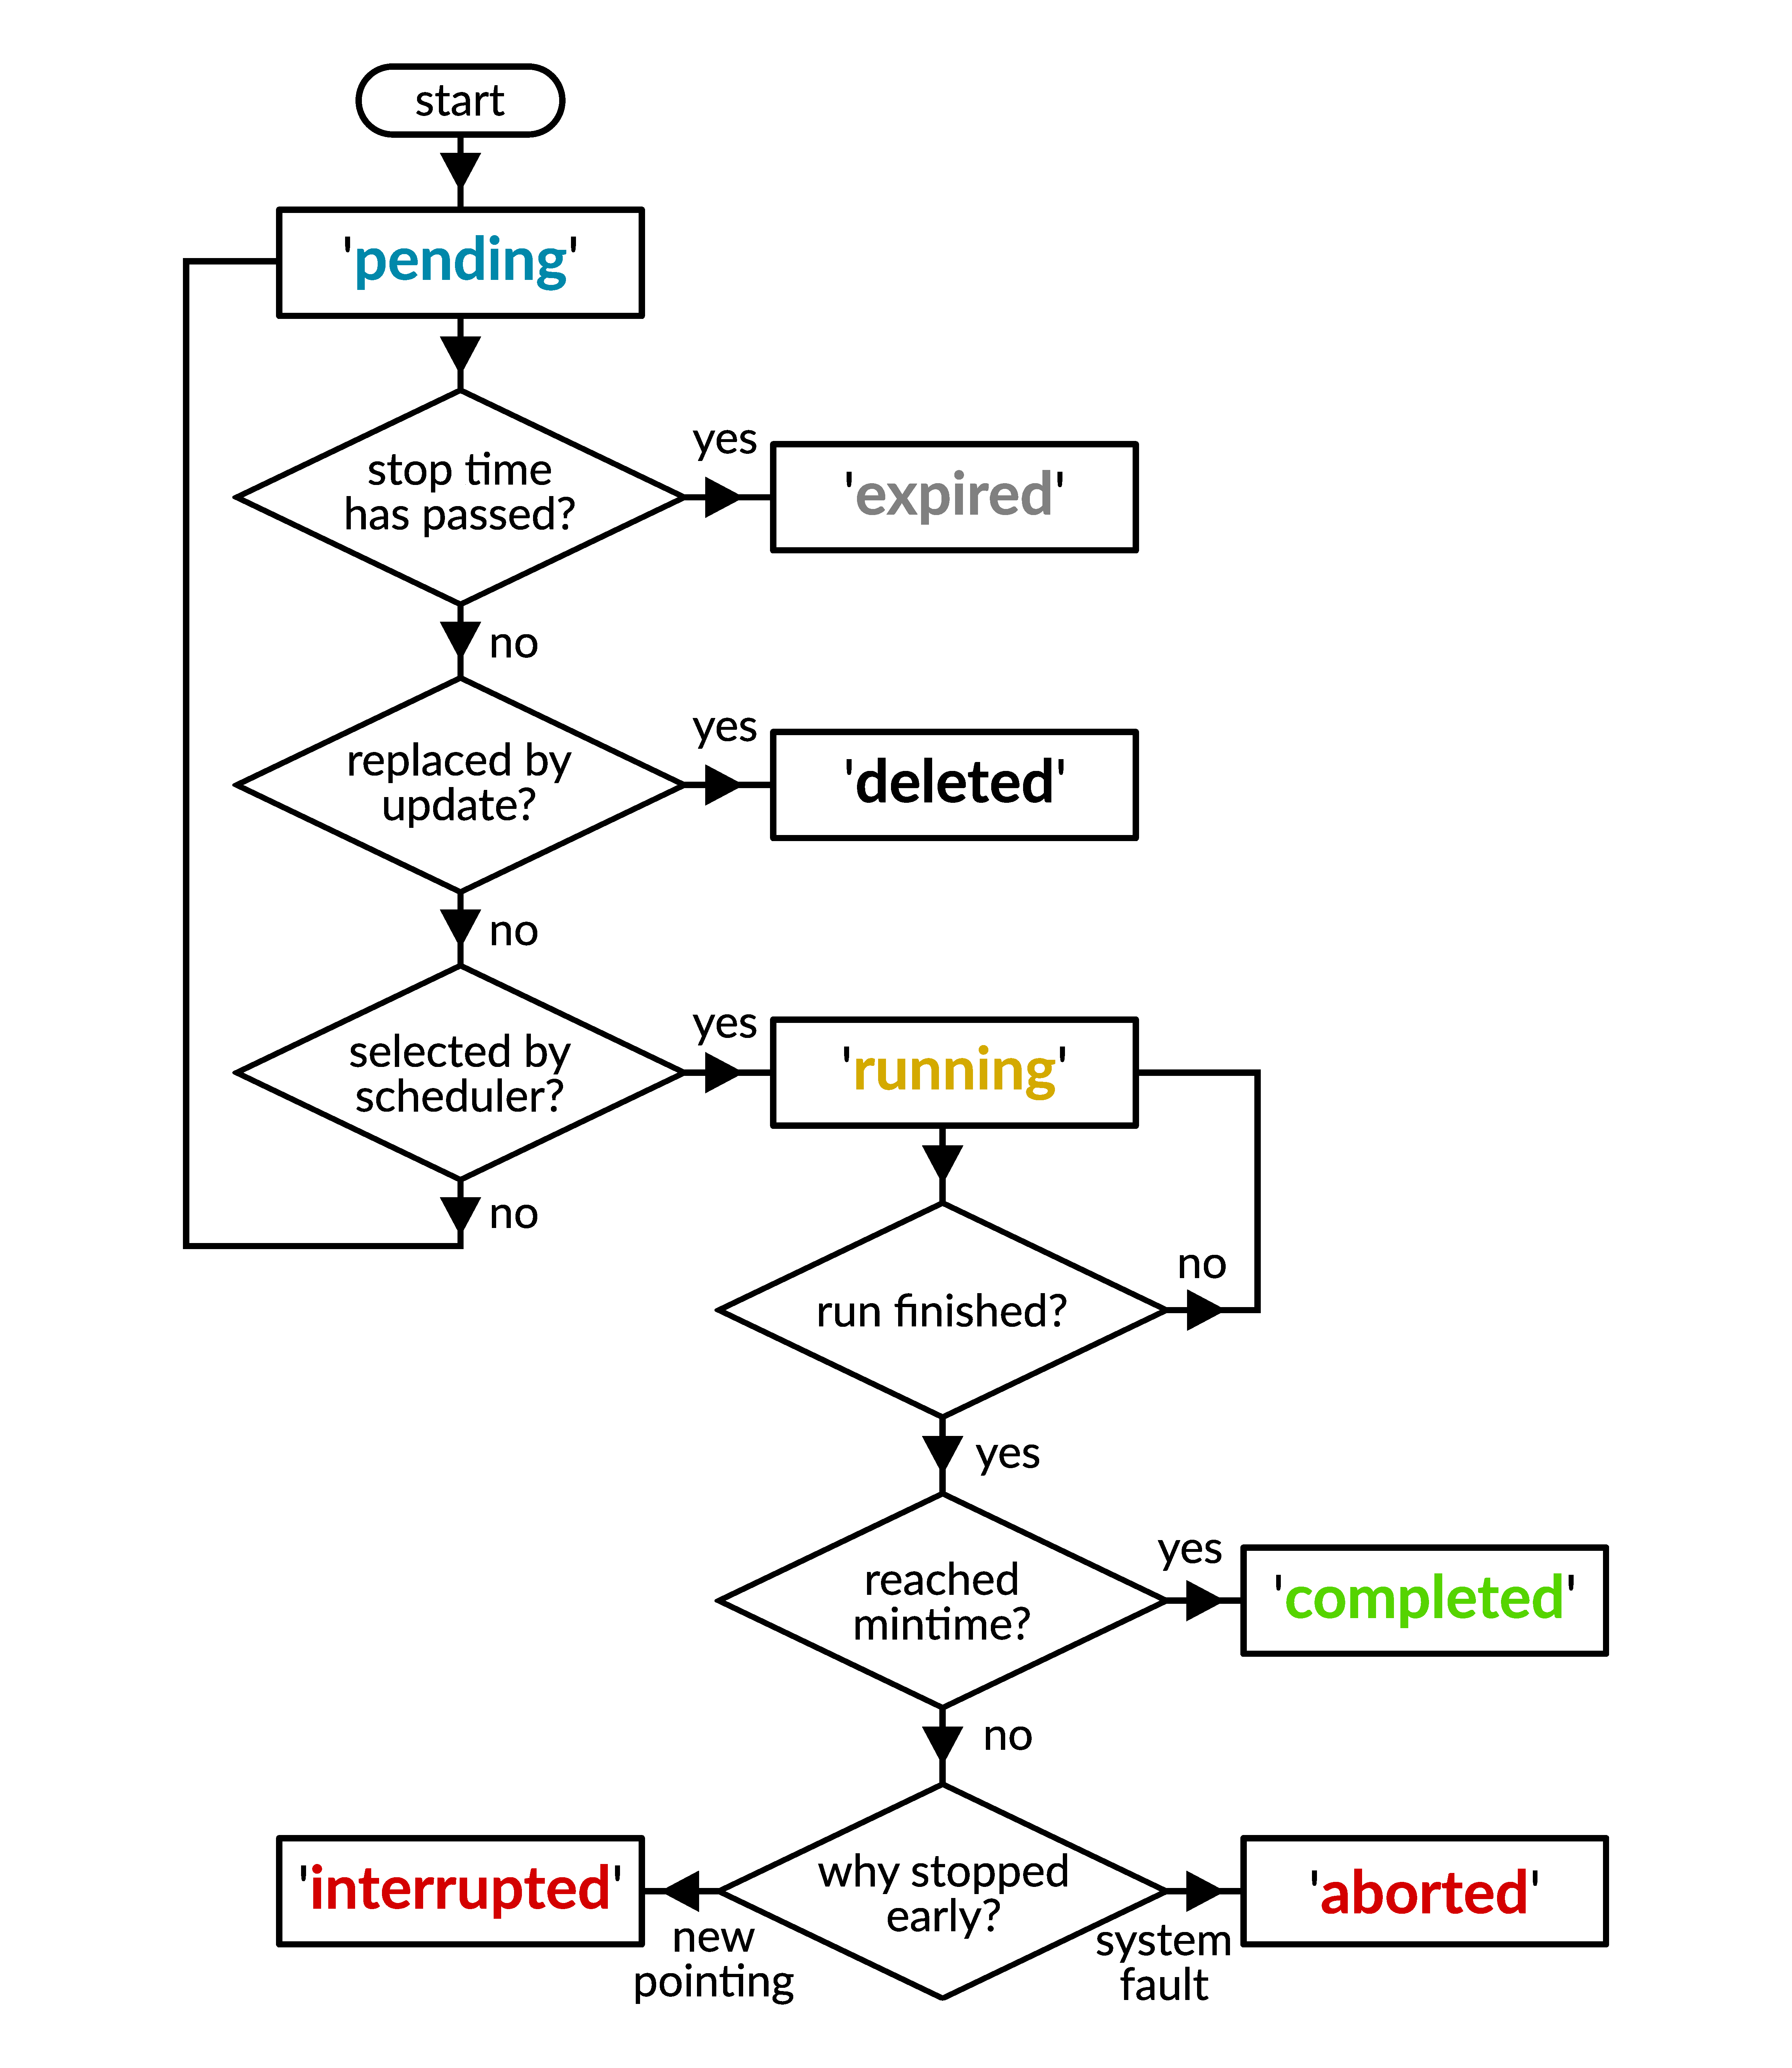
\includegraphics[width=0.9\linewidth]{images/pointings_flowchart.pdf}
    \end{center}
    \caption[Pointing status progression flowchart]{
        A flowchart showing how the status of an entry in the pointings table can change.
    }\label{fig:pointings}
\end{figure}

\clearpage

As well as the target information (RA, Dec, name) a pointing entry contains constraints on when they can be observed. Each pointing can have set start and stop times; the scheduler will only select pointings where the current time is within their valid range (and once the stop time has passed they will be marked as \code{expired}). Limits can also be set on minimum target altitude, minimum distance from the Moon, maximum Moon brightness (in terms of Bright/Grey/Dark time) and maximum Sun altitude. These constraints are applied by the scheduler to each pointing when deciding which to observe, and unless they all pass the pointing is deemed invalid (see \aref{sec:scheduler}). When created, a pointing is also assigned a rank, usually from 0--9, as well as a True/False flag marking it as a time-critical Target of Opportunity (ToO). These are used when calculating the priority of the pointing, to compare with others in order to determine which is the highest priority to observe.

The commands to be executed once the telescope has slewed to a pointing are stored in a separate \code{exposure\_sets} table. An exposure set defines what commands the pilot will give to the exposure queue daemon (see \aref{sec:exq}). The table has columns for the number of exposures to take, the exposure time and the filter to use. For example an observation requiring three \SI{60}{\second} exposures in the \textit{L} filter followed by one each in the \textit{R}, \textit{G} and \textit{B} filters would require four entries in the table: each with exposure time of \SI{60}{\second}, the first with number of exposures as 3 and filter as \textit{L} and the rest with number of exposures as 1 and the individual filters. When the pointing is observed by the pilot will add the linked exposure sets to the queue, and each will then be observed in turn.

Each entry in the pointings table can only be observed once. For observing a target more than once there also exists the \code{mpointings} table, which contains information to dynamically re-generate pointings for a given target. An mpointing entry is defined with three key values: the requested number of observations, the time each should be valid in the queue and the time to wait between each observation. Each time the database caretaker script is run it looks for any entries in the mpointing table that still have observations to do and it creates another entry in the pointings table for that target. Setting the time values allows a lot of control over when pointings can be valid, for example scheduling follow-up observations a set number of hours or days after an initial pointing is observed.

The three tables described above (\code{pointings}, \code{exposure\_sets} and \code{mpointings}) are the core tables required for observation scheduling. However there are other tables defined in the database which are used to group pointings together and relate to GOTO's purpose as a survey instrument. As described in more detail in \aref{sec:gototile}, GOTO observes the sky divided into a fixed grid of individual tiles. The database therefore also contains a \code{grids} table and a \code{grid\_tiles} table, which define the current grid based on the field of view of the telescope. Mapping pointings to the grid is achieved through two more tables, \code{surveys} and \code{survey\_tiles}. A \textit{survey} in this context is a group of tiles that are being observed for a specific reason, one example are the pointings comprising the all-sky survey that \gls{goto} carries out every night. Events that are processed by the alert sentinel (see \aref{sec:sentinel}) might have a skymap that covers multiple tiles, and therefore the set of pointings required to cover it forms a survey within the database. Each pointing within the survey is linked to a survey tile, and each survey tile is linked to a grid tile of the current grid. The additional field added by the survey tile is a `weighting' column, which allows tiles within a survey to be weighted relative to each other. In the all-sky survey each tile is weighted equally, but in a survey coming from an event skymap the tiles will be weighted by the contained probability within that tile. The scheduler takes this weighting into account when deciding which pointing to observe (see \aref{sec:scheduler}, and \aref{sec:scheduler_sims} for more details).

There are two additional tables that are used to contain supporting information: the \code{events} and \code{users} tables. The \code{events} table contains fields such as the event type and source, and is filled by the sentinel when events are processed (see \aref{sec:sentinel}). The \code{users} table connects each pointing to the user who added it to the database. At the moment this is unused, and each pointing is linked to the single generic ``GOTO'' user, but in the future individuals might wish to insert and keep track of their own targets.

\end{colsection}

% ~~~~~~~~~~~~~~~~~~~~

\subsection{The sentinel}
\label{sec:sentinel}
\begin{colsection}

In order for targets to be observed by GOTO in robotic mode they must have entries defined in the \code{pointings} table in the observation database (see \aref{sec:obsdb}). These can be added manually, but for automated observation they have to be inserted whenever an alert is detected. This is the job of the sentinel daemon, as shown in \aref{fig:flow}.

In addition the normal control loop, the sentinel daemon includes an independent alert listener loop that is continuously monitoring the transient alert stream outputted by the 4 Pi Sky event broker \citep{4pisky}, using functions from the PyGCN (\pkg{pygcn}) Python package\footnote{\url{https://pypi.org/project/pygcn/}}. Should the link to the 4 Pi Sky server fail then the daemon will automatically attempt to re-establish the connection every few seconds until it is restored. Alerts come in to the listener in the form of VOEvents \citep{voevent}, and pending alerts are appended to an internal queue before being processed using the event handler defined in the Python module GOTO-alert (\pkg{gotoalert}, see \aref{sec:gotoalert}). The sentinel also has an additional \code{ingest} command which can be used to manually insert test events or bypass the alert listener. The details of how alerts are processed are described in \aref{chap:alerts}, which includes details on how VOEvents are processed, mapped onto the GOTO all-sky grid and added to the database.

The alert listener is a key part of the automated system but was not initially planned to be assigned to its own independent daemon. The \gls{pt5m} system uses the Comet software \citep{comet} in a separate script independent of any daemons. The advantages to including a dedicated alert listener daemon in G-TeCS, which became known as the sentinel, come from it being integrated into the pilot monitoring systems like the other daemons (described in \aref{sec:pilot}). Should the sentinel daemon crash or not respond to checks the pilot will notice and restart it like any other daemon.

\end{colsection}

% ~~~~~~~~~~~~~~~~~~~~

\subsection{The scheduler}
\label{sec:scheduler}
\begin{colsection}

\todo{Need to link to new \aref{chap:scheduling}}

In order for a target to be observed by the telescope in robotic mode an appropriate pointing must be added to the observation database (or an ``mpointing'' entry that generates pointings, as described in \aref{sec:obsdb}). These can be added manually if desired, but in most cases they are either defined once when the database is created (for the constant all-sky survey tiles) or added by the sentinel daemon when a transient alert is received. All entries in the \code{pointings} table with status ``\code{pending}'' form the current \textit{queue}, and the task of selecting which of these pointings the system should observe is the role of the scheduler.

Within \gls{gtecs} the \textit{scheduler} can refer to two linked concepts: the scheduling functions or the scheduler daemon itself (which is often just called ``the'' scheduler, like the sentinel). In the \gls{pt5m} system there is no independent ``scheduler'' daemon, and when the pilot needs to know what to observe it simply calls the scheduling functions to read the current queue, rank the pointings and find the one with the highest priority. When expanding the system for \gls{goto} it was decided to farm these calculations off to a separate daemon, which the pilot instead queries just like the other hardware daemons. There are several advantages to this method. Firstly the scheduling commands can take a significant amount of time (several seconds), so splitting this out to a separate program saves time and frees up the pilot thread for other routines (recall the pilot is asynchronous but not multi-threaded). Secondly separating out the scheduling to an independent daemon allows it to be run on a different computer to the pilot. As shown in \aref{fig:flow} the scheduler daemon runs on the same central server in SuperWASP that hosts the observing database (see \aref{sec:obsdb}), which improves the speed of the database queries. The central server is also simply a more powerful machine than the NUC in the dome that runs the pilot and other hardware daemons, which also reduces the time to run the queries. Finally, when GOTO moves to a multi-telescope system it is anticipated that the scheduler will be one of the common systems shared between telescopes (see \aref{sec:gtecs_multisite}), and so it makes sense to have the scheduler daemon on the central server alongside the other shared systems.

The scheduler daemon contains the usual control loop, which runs the scheduling functions described below and internally stores the returned highest-priority pointing. The daemon exposes a single command, \code{check\_queue}, which returns the ID of that pointing. The pilot \code{check\_schedule} coroutine queries the daemon every 10 seconds using this command, and the scheduler returns one of three results: carry on with the current observation, switch to a new observation, or park the telescope (in the case that there are no valid targets). Most of the time the pilot will be observing a pointing previously given by the scheduler, and on the next check the scheduler will return the same pointing as it is still the highest priority --- in which case pilot will continue observing it. Even if the scheduler finds that a different pointing now has a higher priority it will not tell the pilot to change targets whilst observing the current target, unless the new pointing has the \glsfirst{too} flag set. Otherwise the pilot will wait until it has finished the current job, mark it as complete in the database and ask the scheduler for the next target to observe. The different cases are summarised in \aref{tab:sched}.

%\begin{landscape}
%\begin{table}[p]

\begin{sidewaystable}[p]
    \begin{center}
        \begin{tabular}{cc|cccc} % chktex 44
            &
            & \multicolumn{4}{c}{Highest priority pointing is\ldots}
            \\[0.5cm]
            &
            & \makecell{\ldots same as \\ current pointing}
            & \makecell{\ldots a new, \\ valid pointing}
            & \makecell{\ldots a new, \\ invalid pointing}
            & \ldots None
            \\[0.5cm]
            \midrule
            & & & & &
            \\
            \multirow{8}{*}{\rotatebox[origin=c]{90}{Current pointing is\ldots}}
            & \ldots valid
            & \makecell{\textcolor{Green}{Continue} \\ \textcolor{Green}{current pointing}}
            & \makecell{\textcolor{BlueGreen}{Interrupt and start new pointing} \\ \textcolor{BlueGreen}{if it is a ToO and the current pointing is not,} \\ \textcolor{BlueGreen}{otherwise continue current pointing}}
            & \textcolor{Red}{Park}
            & \textcolor{Red}{Park}
            \\[1.5cm]
            & \ldots invalid
            & \textcolor{Red}{Park}
            & \textcolor{NavyBlue}{Interrupt and start new pointing}
            & \textcolor{Red}{Park}
            & \textcolor{Red}{Park}
            \\[1.5cm]
            & \ldots N/A (parked)
            & \textcolor{Red}{Remain parked}
            & \textcolor{NavyBlue}{Unpark and start new pointing}
            & \textcolor{Red}{Remain parked}
            & \textcolor{Red}{Remain parked}
            \\[0.5cm]
        \end{tabular}
    \end{center}
    \caption[Actions to take based on scheduler results]{
        Actions the pilot will take based on the scheduler results. The scheduler can return one of three options as the highest priority pointing: the current pointing, a different pointing or \code{None} (meaning the current queue is empty). Each pointing can either be valid or invalid. The pilot will either continue with the current pointing (\textcolorbf{Green}{green}), switch to the new pointing depending on the ToO flag (\textcolorbf{NavyBlue}{blue}, \textcolorbf{BlueGreen}{blue-green}) or park the telescope (\textcolorbf{Red}{red}).
    }\label{tab:sched}
\end{sidewaystable}

%\end{table}
%\end{landscape}

\end{colsection}

% ~~~~~~~~~~~~~~~~~~~~

\end{colsection}

% ########################################
